%----------------------------------------------------------------------------------------
%	PACKAGES AND THEMES
%----------------------------------------------------------------------------------------
\documentclass[aspectratio=169,xcolor=dvipsnames]{beamer}
\usetheme{Simple}
\usepackage[T1,T2A]{fontenc}
\usepackage[utf8]{inputenc}
\usepackage[english,russian]{babel}
\usepackage{hyperref}
\usepackage{graphicx} % Allows including images
\usepackage{booktabs} % Allows the use of \toprule, \midrule and \bottomrule in tables


\newcommand{\eqdef}{\; { := }\;}
\newcommand{\R}{\mathbb{R}}
\newcommand{\Exp}{\mathbb{E}}
\newcommand{\ExpBr}[1]{\mathbb{E}\left[#1\right]}
\newcommand{\norm}[1]{\left\|#1\right\|}
\def\<#1,#2>{\langle #1,#2\rangle}
\newcommand{\cX}{\mathcal{X}}
\newcommand{\bJ}{\mathbf{J}}
\newcommand{\dom}{\operatorname{dom}}
\newcommand{\prox}{\operatorname{prox}}
\newcommand{\footeq}[1]{{\footnotesize #1}}

\newcommand{\newalpha}{h}

\usepackage{tcolorbox}
\usepackage{pifont}
\definecolor{mydarkgreen}{RGB}{39,130,67}
\definecolor{mydarkred}{RGB}{192,47,25}
\newcommand{\green}{\color{mydarkgreen}}
\newcommand{\red}{\color{mydarkred}}
\newcommand{\cmark}{\green\ding{51}}%
\newcommand{\xmark}{\red\ding{55}}%

\newcommand{\mA}{\mathbf{A}}
\newcommand{\mB}{\mathbf{B}}
\newcommand{\mC}{\mathbf{C}}
\newcommand{\mH}{\mathbf{H}}
\newcommand{\mI}{\mathbf{I}}
\newcommand{\mU}{\mathbf{U}}
\newcommand{\mZ}{\mathbf{Z}}

\newcommand{\cC}{{\mathcal{C}}}
\newcommand{\cH}{{\mathcal{H}}}

\newtheorem{def1}{Определение}

%----------------------------------------------------------------------------------------
%	TITLE PAGE
%----------------------------------------------------------------------------------------

% The title
\title[short title]{Распределенные методы второго порядка с быстрой скоростью сходимости и компрессией}

\author[Rustem] {Исламов Рустем}
\institute[NTU] % Your institution may be shorthand to save space
{
    % Your institution for the title page
    Московский физико-технический институт\\
    Кафедра Интеллектуальных систем\\
    \vskip 10pt
    Научный руководитель: д.ф.-м.н. Стрижов В.В.
}
\date{Апрель, 2021} % Date, can be changed to a custom date


%----------------------------------------------------------------------------------------
%	PRESENTATION SLIDES
%----------------------------------------------------------------------------------------

\begin{document}

\begin{frame}
    % Print the title page as the first slide
    \titlepage
\end{frame}

%\begin{frame}{Постановка задачи}
    % Throughout your presentation, if you choose to use \section{} and \subsection{} commands, these will automatically be printed on this slide as an overview of your presentation
%    \tableofcontents
%\end{frame}

%------------------------------------------------
%\section{First Section}
%------------------------------------------------

\begin{frame}{Постановка задачи}
    \begin{block}{Оптимизационная задача}
        Определить оптимальные параметры модели машинного обучения путем решения оптимизационной задачи:
        \begin{equation}
            \min\limits_{x\in \R^d}\left\{P(x) \eqdef f(x) + \frac{\lambda}{2}\|x\|^2\right\},
        \end{equation}
        где $x$~--- параметры модели, а $f$~--- функция потерь.
    \end{block}
    Предполагается, что данные для обучения распределены между $n$ клиентами, каждый клиент $i \in \{1,\dots,n\}$ имеет доступ к $m$ векторам признаков объектов $a_{ij}\in \R^d$, $j\in \{1,\dots,m\}$. Функция $f$ имеет вид
    \begin{equation}
        f(x) = \frac{1}{n}\sum\limits_{i=1}^n f_i(x), \qquad f_i(x) = \frac{1}{m}\sum\limits_{j=1}^m f_{ij}(x), \qquad f_{ij}(x) = \varphi_{ij}(a_{ij}^\top x).
    \end{equation}
\end{frame}

\begin{frame}{Работы по теме}
    \begin{thebibliography}{99} % Beamer does not support BibTeX so references must be inserted manually as below
    
    \bibitem \ Konstantin Mishchenko, Eduard Gorbunov, Martin Takac, and Peter Richtarik. 
    \newblock \textit{Distributed learning with compressed gradient differences.}
    \newblock arXiv:1901.09269, 2019.
    \\
    \bibitem Z Zhize Li, Dmitry Kovalev, Xun Qian, and Peter Richtarik.
    \newblock \textit{Acceleration for compressed
gradient descent in distributed and federated optimization.}
    \newblock In International Conference on Machine Learning, 2020.
    \\
    \bibitem R Rixon Crane and Fred Roosta.
    \newblock \textit{DINGO: Distributed Newton-type method
for gradient-norm optimization.}
    \newblock Advances in Neural Information Processing Systems, volume 32, pages 9498.
    \\
    \bibitem c Rustem Islamov, Xun Qian, and Peter Richtarik.
    \newblock \textit{Distributed second order methods
with fast rates and compressed communication.}
    \newblock arXiv:2102.07158, 2021.


\end{thebibliography}
\end{frame}

\begin{frame}{Модель распределенной оптимизации}
\begin{minipage}[h]{0.65\linewidth}
\begin{block}{Достоинства и недостатки модели}
    \begin{itemize}
        \item[$+$] Возможно обучать модели на больших объемах данных, распределенных между устройствами;
        \item[$+$] Возможно параллелизовать вычисления на устройствах;
        \item[$-$] Скорость обмена данными между Клиентом и Сервером намного медленнее, чем скорость вычислений на самих устройствах и сервере.
    \end{itemize}
\end{block}
\end{minipage}
\hfill
\begin{minipage}[h]{0.32\linewidth}
\begin{center}

\includegraphics[width=0.8\linewidth]{client-server-architecture.png}\\
{\scriptsize Архитектура модели <<Клиент-Сервер>>.}
\end{center}
\end{minipage}


\end{frame}


\begin{frame}{Мотивация}
    \begin{block}{Существующие подходы и их недостатки}
        \begin{itemize}
            \item Скорость сходимости методов первого порядка зависит от числа обусловленности поставленной оптимизационной задачи;
            \item Скорость сходимости методов второго порядка зависит от числа обусловленности поставленной оптимизационной задачи;
            \item Стоимость коммуникации между сервером и клиентом для методов второго порядка очень дорогая.
        \end{itemize}
    \end{block}
    \begin{alertblock}{Цель}
        Предложить эффективный с точки зрения коммуникации метод второго порядка, чья скорость сходимости не зависит от числа обусловленности.
    \end{alertblock}
\end{frame}

\begin{frame}{Предположения и структура Гессианов}
    \begin{block}{Предположение}
        Поставленная оптимизационная задача имеет хотя бы одно решение $x^*$. Для всех $i, j$ функция потерь $\varphi_{ij}:\R\to \R$ является дважды непрерывно дифференцируемой функцией с $\nu$-липшецевой второй производной. 
    \end{block}
    \begin{block}{Гессианы функций}
        Гессианы функций $f_{ij}, f_i, f$ соответственно имеют вид
        \begin{eqnarray}
            \mH_{ij}(x) =  \varphi^{\prime\prime}(a_{ij}^\top x)(x)a_{ij}a_{ij}^\top, \quad \mH_i(x)= \frac{1}{m}\sum\limits_{j=1}^m \mH_{ij}(x), \quad \mH(x) = \frac{1}{n}\sum\limits_{i=1}^n \mH_{i}(x).
        \end{eqnarray}
    \end{block}
\end{frame}


\begin{frame}{Основная идея: {\sf NEWTON-STAR}}
    \begin{block}{NEWTON-STAR}
        Предположим, что Серверу известен Гессиан $\mH(x^*)$ функции $f$ в оптимуме. Шаг метода NEWTON-STAR имеет вид:
        \begin{equation}
            x^{k+1} = x^k - \left(\nabla^2P(x^*)\right)^{-1}\nabla P(x^k) = x^k - \left(\mH(x^*)+\lambda\mI\right)^{-1}\left(\frac{1}{n}\sum\limits_{i=1}^n \nabla f_i(x^k)+\lambda x^k\right).
        \end{equation}
    \end{block}

    \begin{block}{Теорема о сходимости NEWTON-STAR}
        Предположим, что $\mH(x^*) \succeq \mu^*\mI, \mu^* \geq 0,$ причем $\mu^*+\lambda > 0.$ Тогда {\sf NEWTON-STAR} сходится локально квадратично
        \begin{equation}
            \norm{x^{k+1}-x^*} \leq\frac{\nu}{2(\mu^*+\lambda)} \left(\frac{1}{nm}\sum\limits_{i=1}^n\sum\limits_{j=1}^m\norm{a_{ij}}^3\right)\norm{x^k-x^*}^2.
        \end{equation}
    \end{block}
\end{frame}

\begin{frame}{Свойства NEWTON-STAR}
    \begin{block}{Достоинства и недостатки NEWTON-STAR}
        \begin{itemize}
            \item Локальная квадратичная сходимость, наследованная от стандартного метода Ньютона;
            \item Стоимость коммуникаций между Сервером и Клиентом $\mathcal{O}(d)$~--- такая же, как и у градиентных методов. Каждый клиент пересылает серверу только градиент $\nabla f_i(x^k)$;
            \item Метод имеет только теоретическую значимость, Гессиан в оптимуме не известен. 
        \end{itemize}
    \end{block}
\end{frame}

\begin{frame}{NEWTON-LEARN}
    \begin{block}{Дополнительные предположения}
        Каждая функция $\varphi_{ij}$ является выпуклой, параметр регуляризации $\lambda$ положительный. 
    \end{block}
    \begin{alertblock}{Основная идея метода}
    Аппроксимируем матрицу $\mH(x^*)$ на шаге $k$ матрицей $\mH^k$ вида
        \begin{equation}
            \mH^k = \left(\frac{1}{n}\sum\limits_{i=1}^n\frac{1}{m}\sum\limits_{j=1}^mh_{ij}^k a_{ij}a_{ij}^\top\right), \quad x^{k+1} = x^k - \left(\mH^k+\lambda\mI\right)^{-1}\left(\frac{1}{n}\sum\limits_{i=1}^n\nabla f_i(x^k) + \lambda x^k\right).
        \end{equation}
    \end{alertblock}
    Требования:
    \begin{itemize}
        \item $h_{ij}^k \to \varphi_{ij}^{\prime\prime}(a_{ij}^\top x^*) \text{ при } k \to \infty$;
        \item обнолвение элементов вектора $h_i^k \eqdef (h_{i1}^k, \dots, h_{im}^k)$ должно быть мало, т.е вектор $h_i^{k+1} - h_i^k$ разрежен.
    \end{itemize}
\end{frame}


\begin{frame}{Механизм обновления коэффицентов}
    
    \begin{def1}
        Рандомизированное отображение $\cC:\R^m \to \R^m$, удовлетворяющее условиям
        \begin{equation}
            \ExpBr{\cC(h)} = h, \qquad \ExpBr{\norm{\cC(h)}^2} \leq (\omega+1)\norm{h}^2, \qquad \forall~h \in \R^m,
        \end{equation}
        называется {\bf оператором несмещенной компрессии.}\\
        {\bf Пример}: оператор Rand-$r$, выходом такого оператора являются случайно выбранные $r$ элементов входа, домноженные на $\frac{m}{r}.$ Для этого оператора параметр $\omega=\frac{m}{r}-1.$
    \end{def1}
    
    Введем $A_i \eqdef (a_{i1}^\top, \dots, a_{im}^\top), \varphi^{\prime\prime}_i(A_ix) \eqdef (\varphi_{i1}^{\prime\prime}(a_{i1}^\top x), \dots, \varphi_{i1}^{\prime\prime}(a_{im}^\top x))^\top.$
    \begin{block}{Механизм обновления (DIANA-trick $[1]$)}
    \begin{equation}
        h_i^{k+1} = \left[h_i^k + \eta \cC^k_i(\varphi_{i}^k(A_ix^k)-h_i^k)\right]_+.
    \end{equation}
    \end{block}
\end{frame}
%------------------------------------------------


\begin{frame}{Сходимость NEWTON-LEARN}
Введем функцию Ляпунова $\Phi^k_1 \eqdef \norm{x^k-x^*}^2 + \frac{1}{3mn\eta \nu^2R^2}\sum\limits_{i=1}^n\norm{h_i^k-\varphi_i^{\prime\prime}(A_ix^*)}^2,$ где $R = \max_{i,j}\norm{a_{ij}}$.

\begin{block}{Теорема о сходимости NEWTON-LEARN}
Пусть $\eta \leq \frac{1}{\omega+1}$ и $\norm{x^k-x^*}^2 \leq \frac{\lambda^2}{12\nu^2R^6}$ для всех $k \geq 0.$ Тогда выполнено
\begin{eqnarray*}
    \ExpBr{\Phi^k_1}  \leq  \theta_1^k \Phi^0_1,\qquad \ExpBr{\frac{\norm{x^{k+1}-x^*}^2}{\norm{x^{k}-x^*}^2}} \leq  \theta_1^k \left(6\eta+\frac{1}{2}\right)\frac{\nu^2R^6}{\lambda^2}\Phi_1^0,
\end{eqnarray*}
где $\theta_1 = 1- \min\left\{\frac{\eta}{2}, \frac{5}{8}\right\}.$
\end{block}
{\bf Лемма:} при использовании оператора разреживания достаточно предположить, что $\norm{x^0-x^*}^2 \leq \frac{\lambda^2}{12\nu^2R^6}.$
\end{frame}

\begin{frame}{Эксперименты}
Эксперименты проведены для логистической регрессии на различных наборах данных библиотке LIBSVM.
\begin{equation}
    P(x) = \frac{1}{nm}\sum\limits_{i=1}^n\sum\limits_{j=1}^m\log\left(1+\exp(-b_{ij}a_{ij}^\top x)\right) + \frac{\lambda}{2}\|x\|^2, \quad a_{ij} \in \R^d, b_{ij} \in \{-1,1\}.
\end{equation}

\begin{tabular}{ccc}
     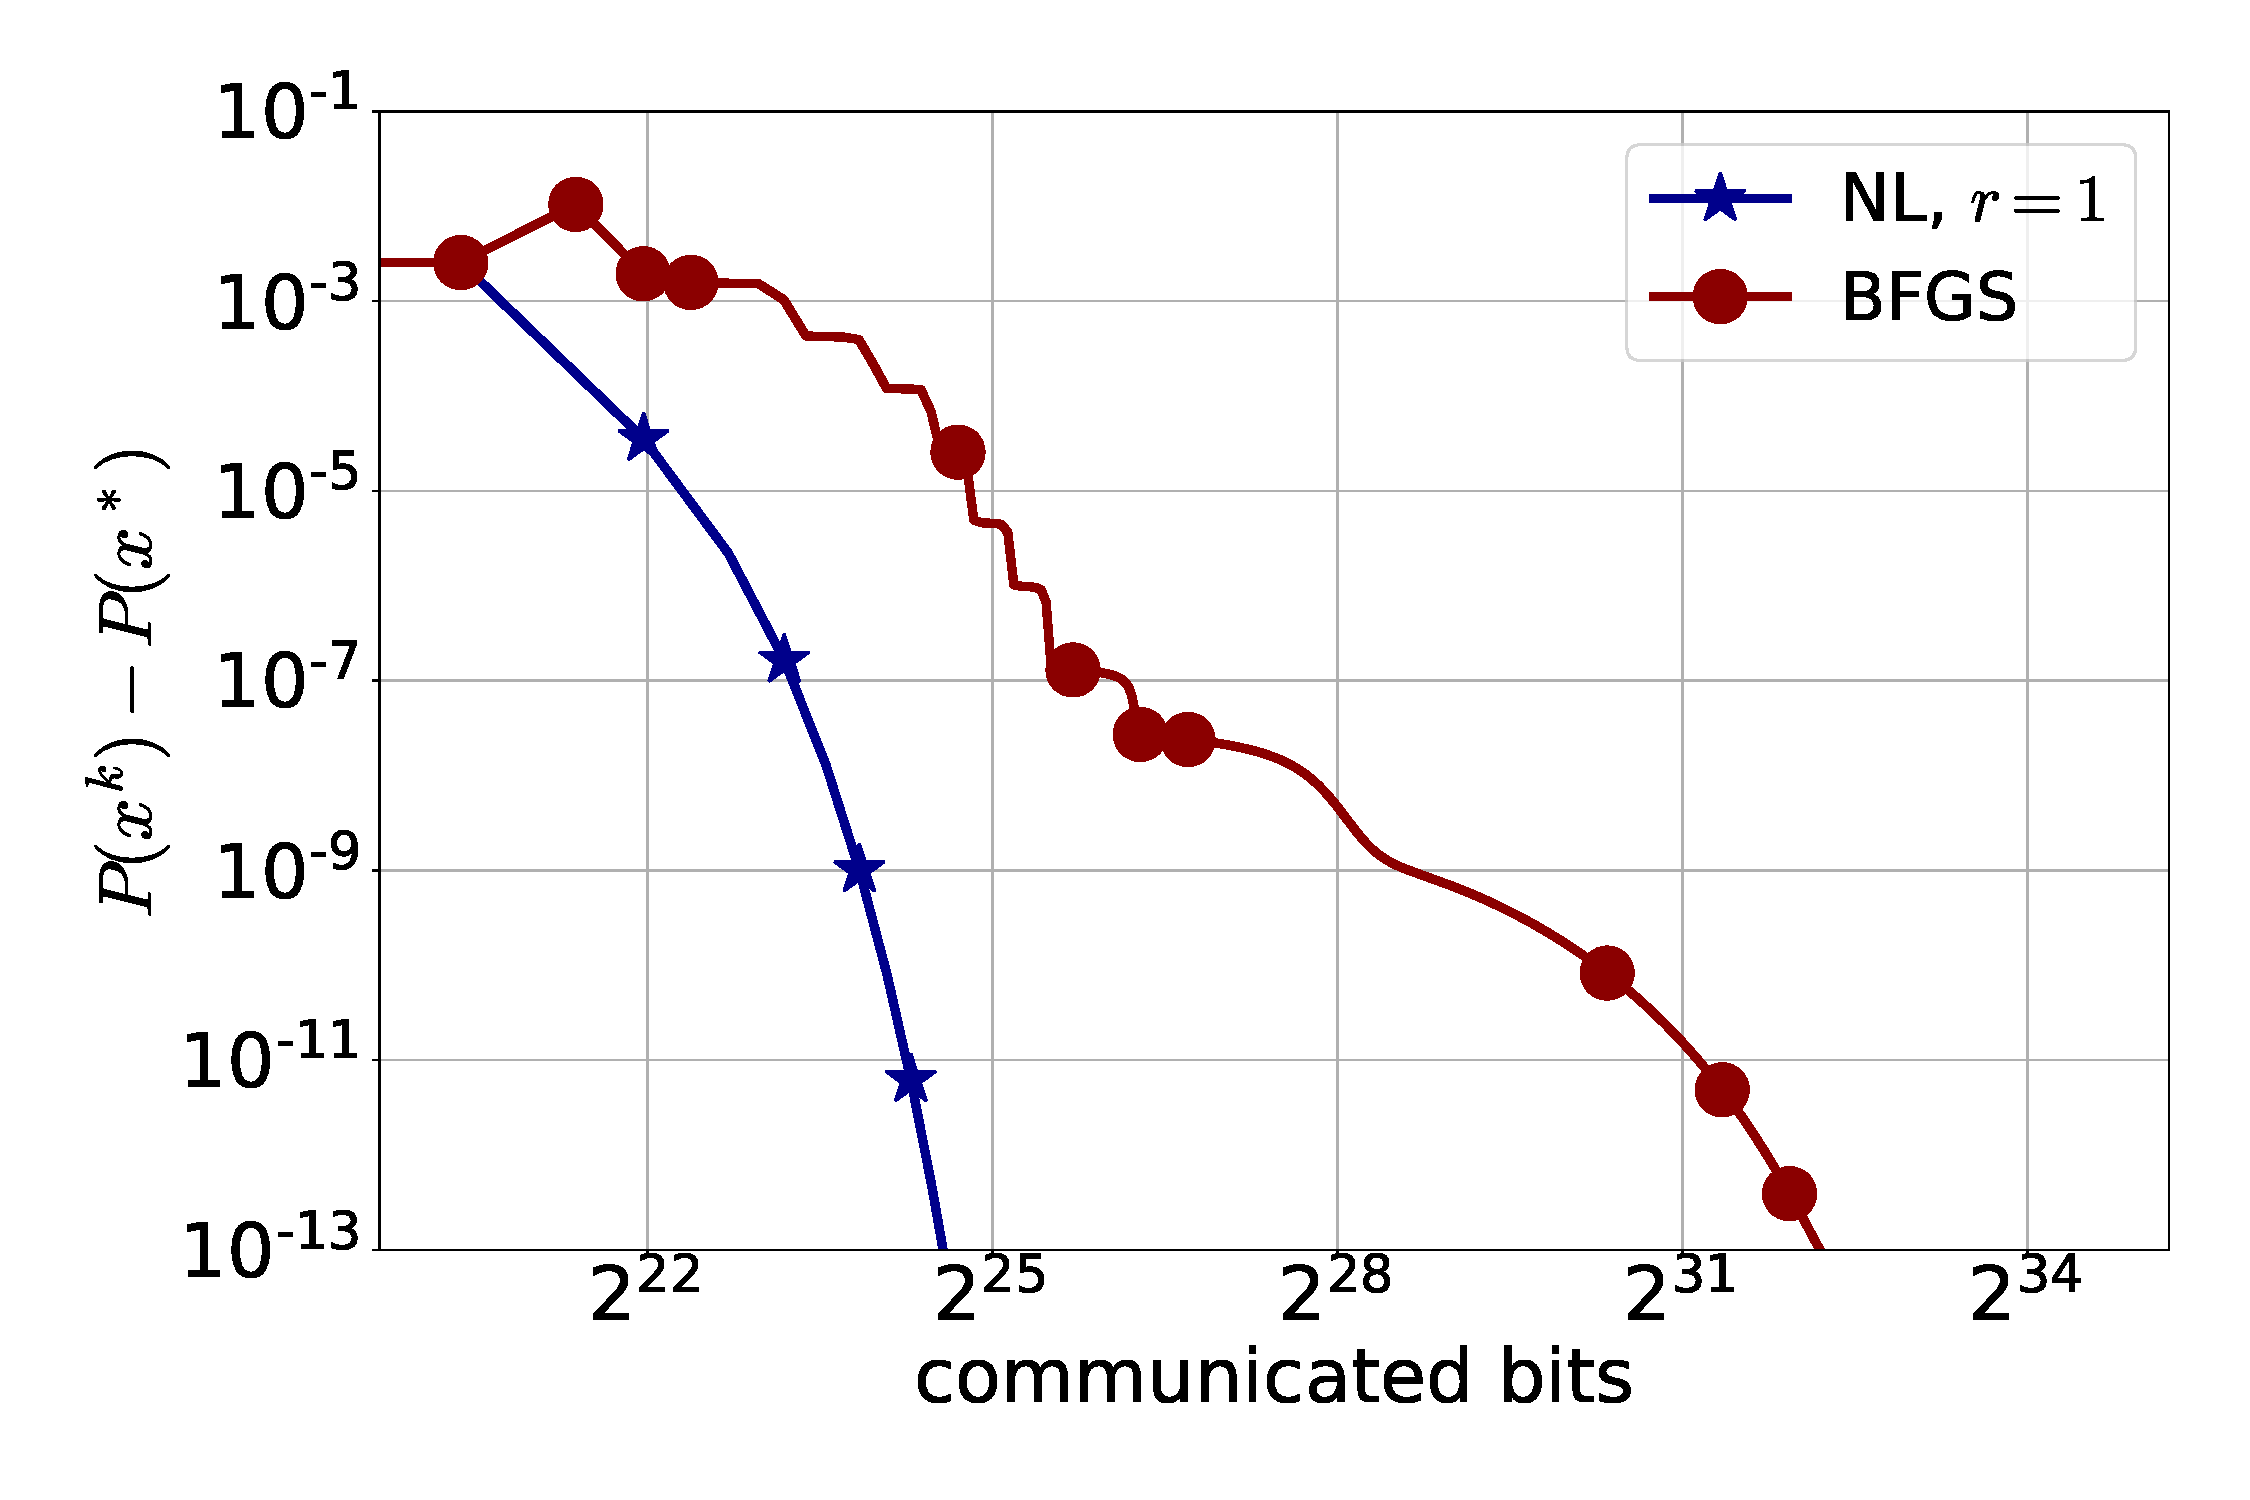
\includegraphics[width=0.3\linewidth]{w8a_nl_bfgs_bits_lmb=0_001.pdf}& 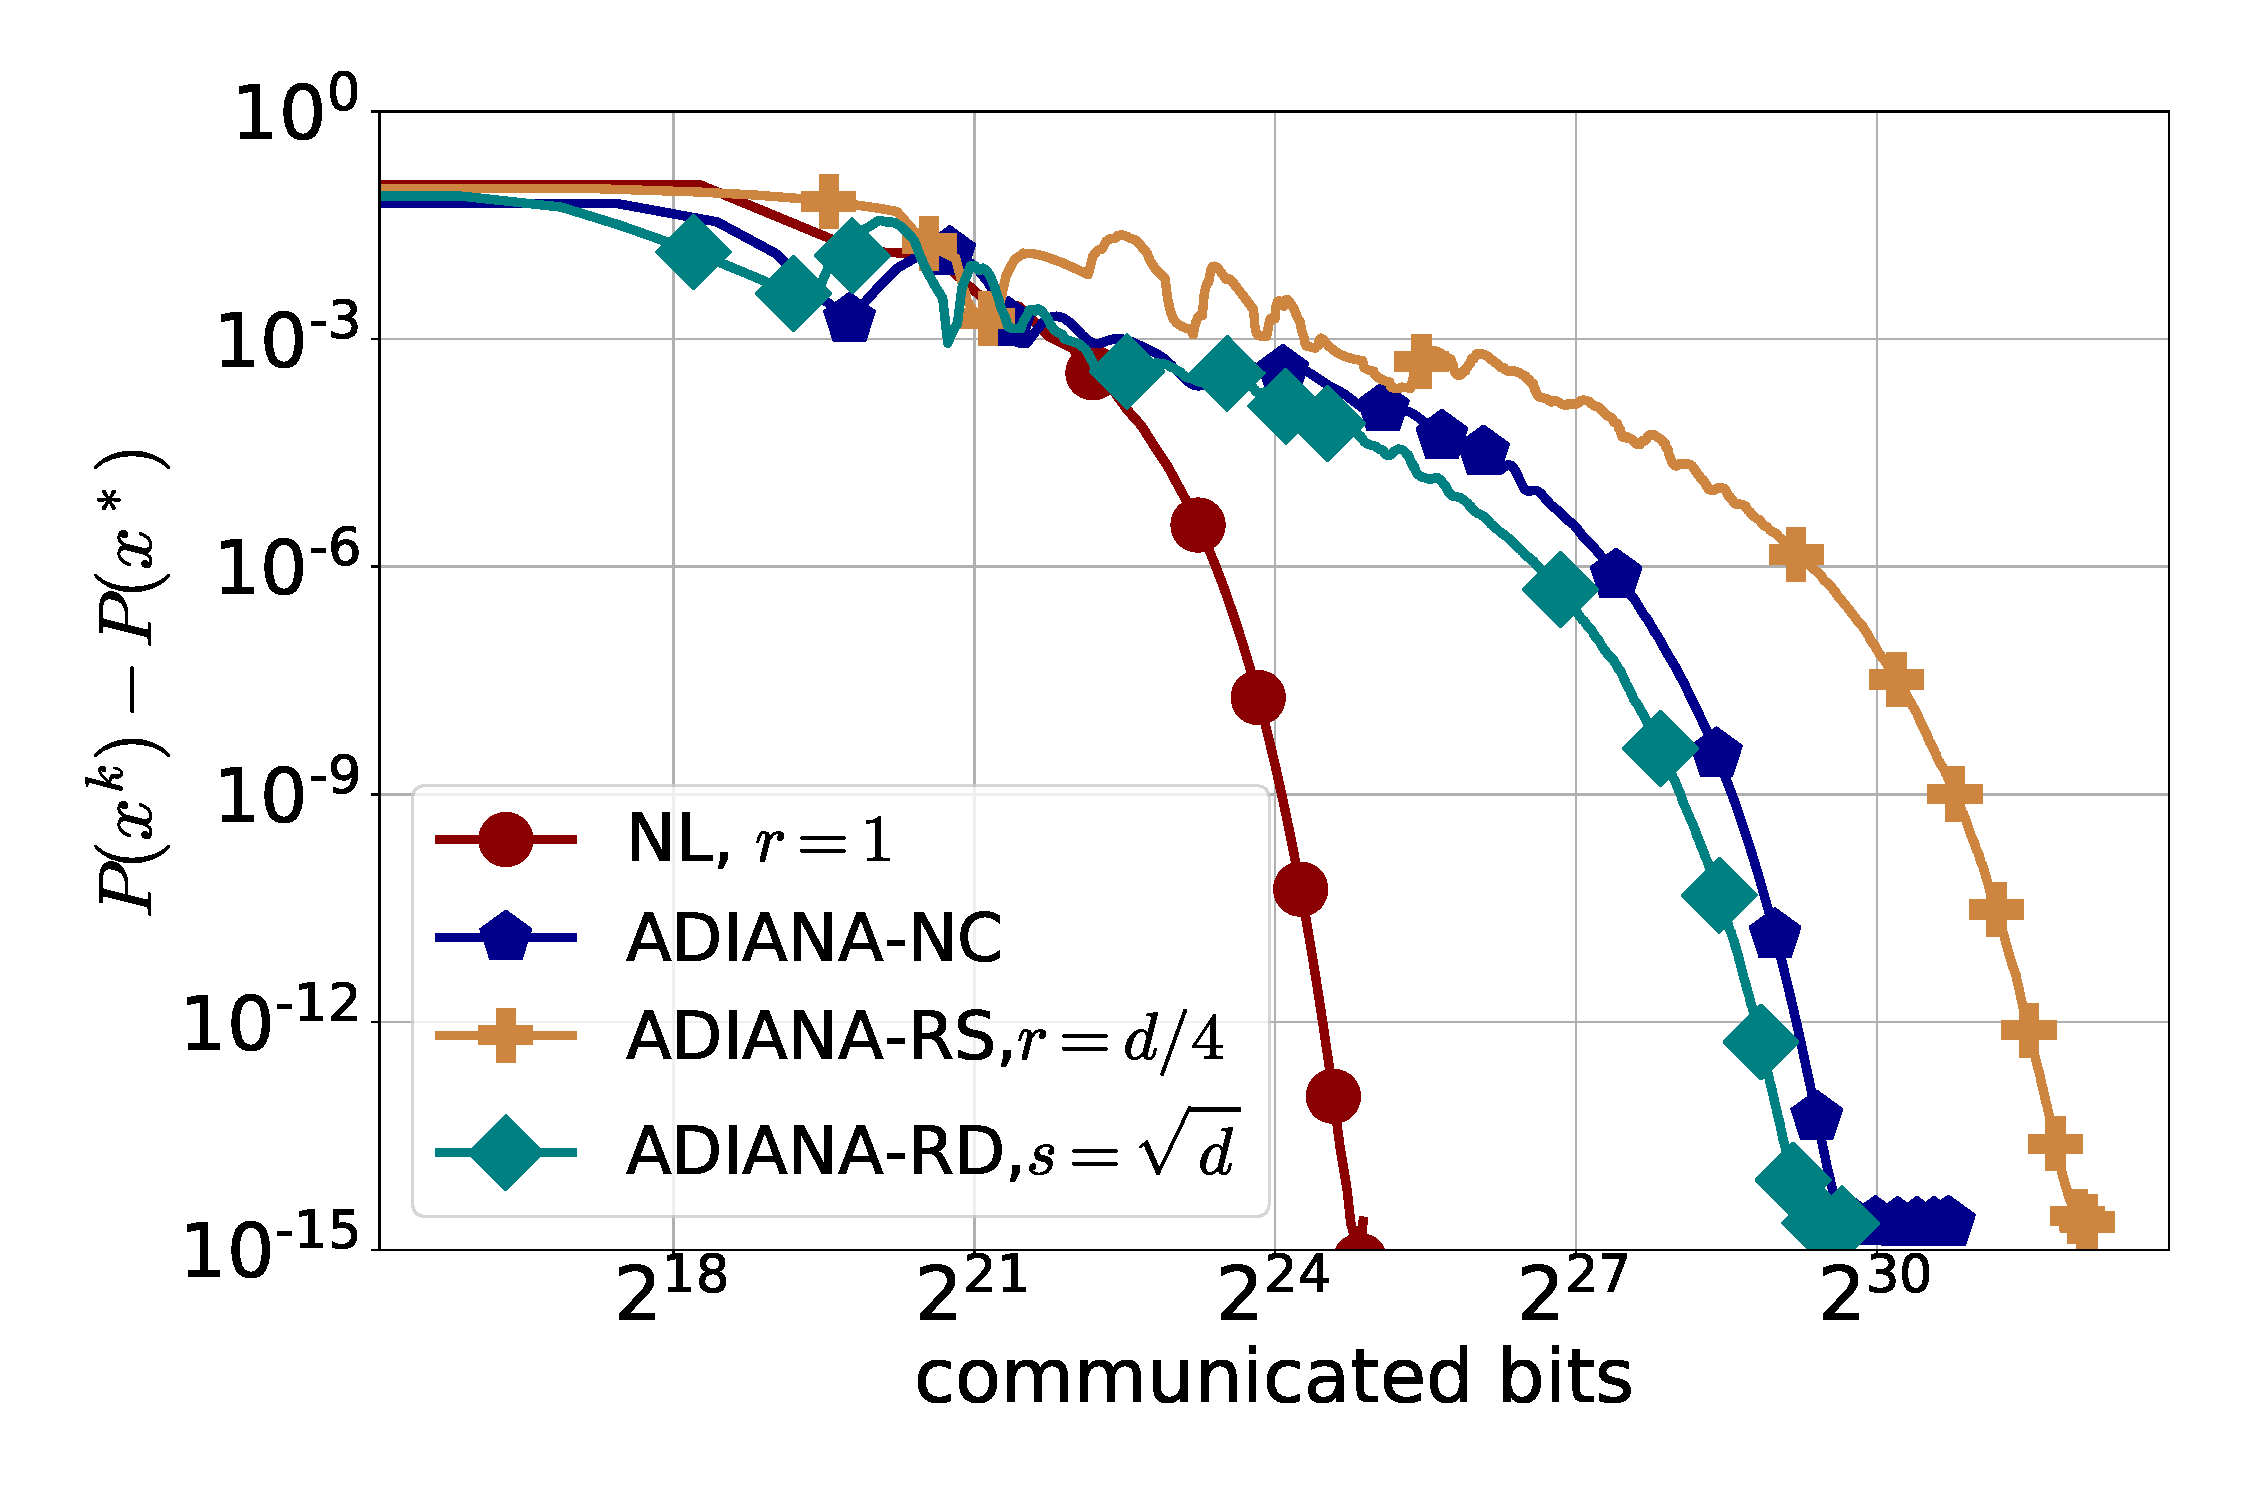
\includegraphics[width=0.3\linewidth]{a9a_nl_adiana_bits_lmb=0_0001.pdf}
     &  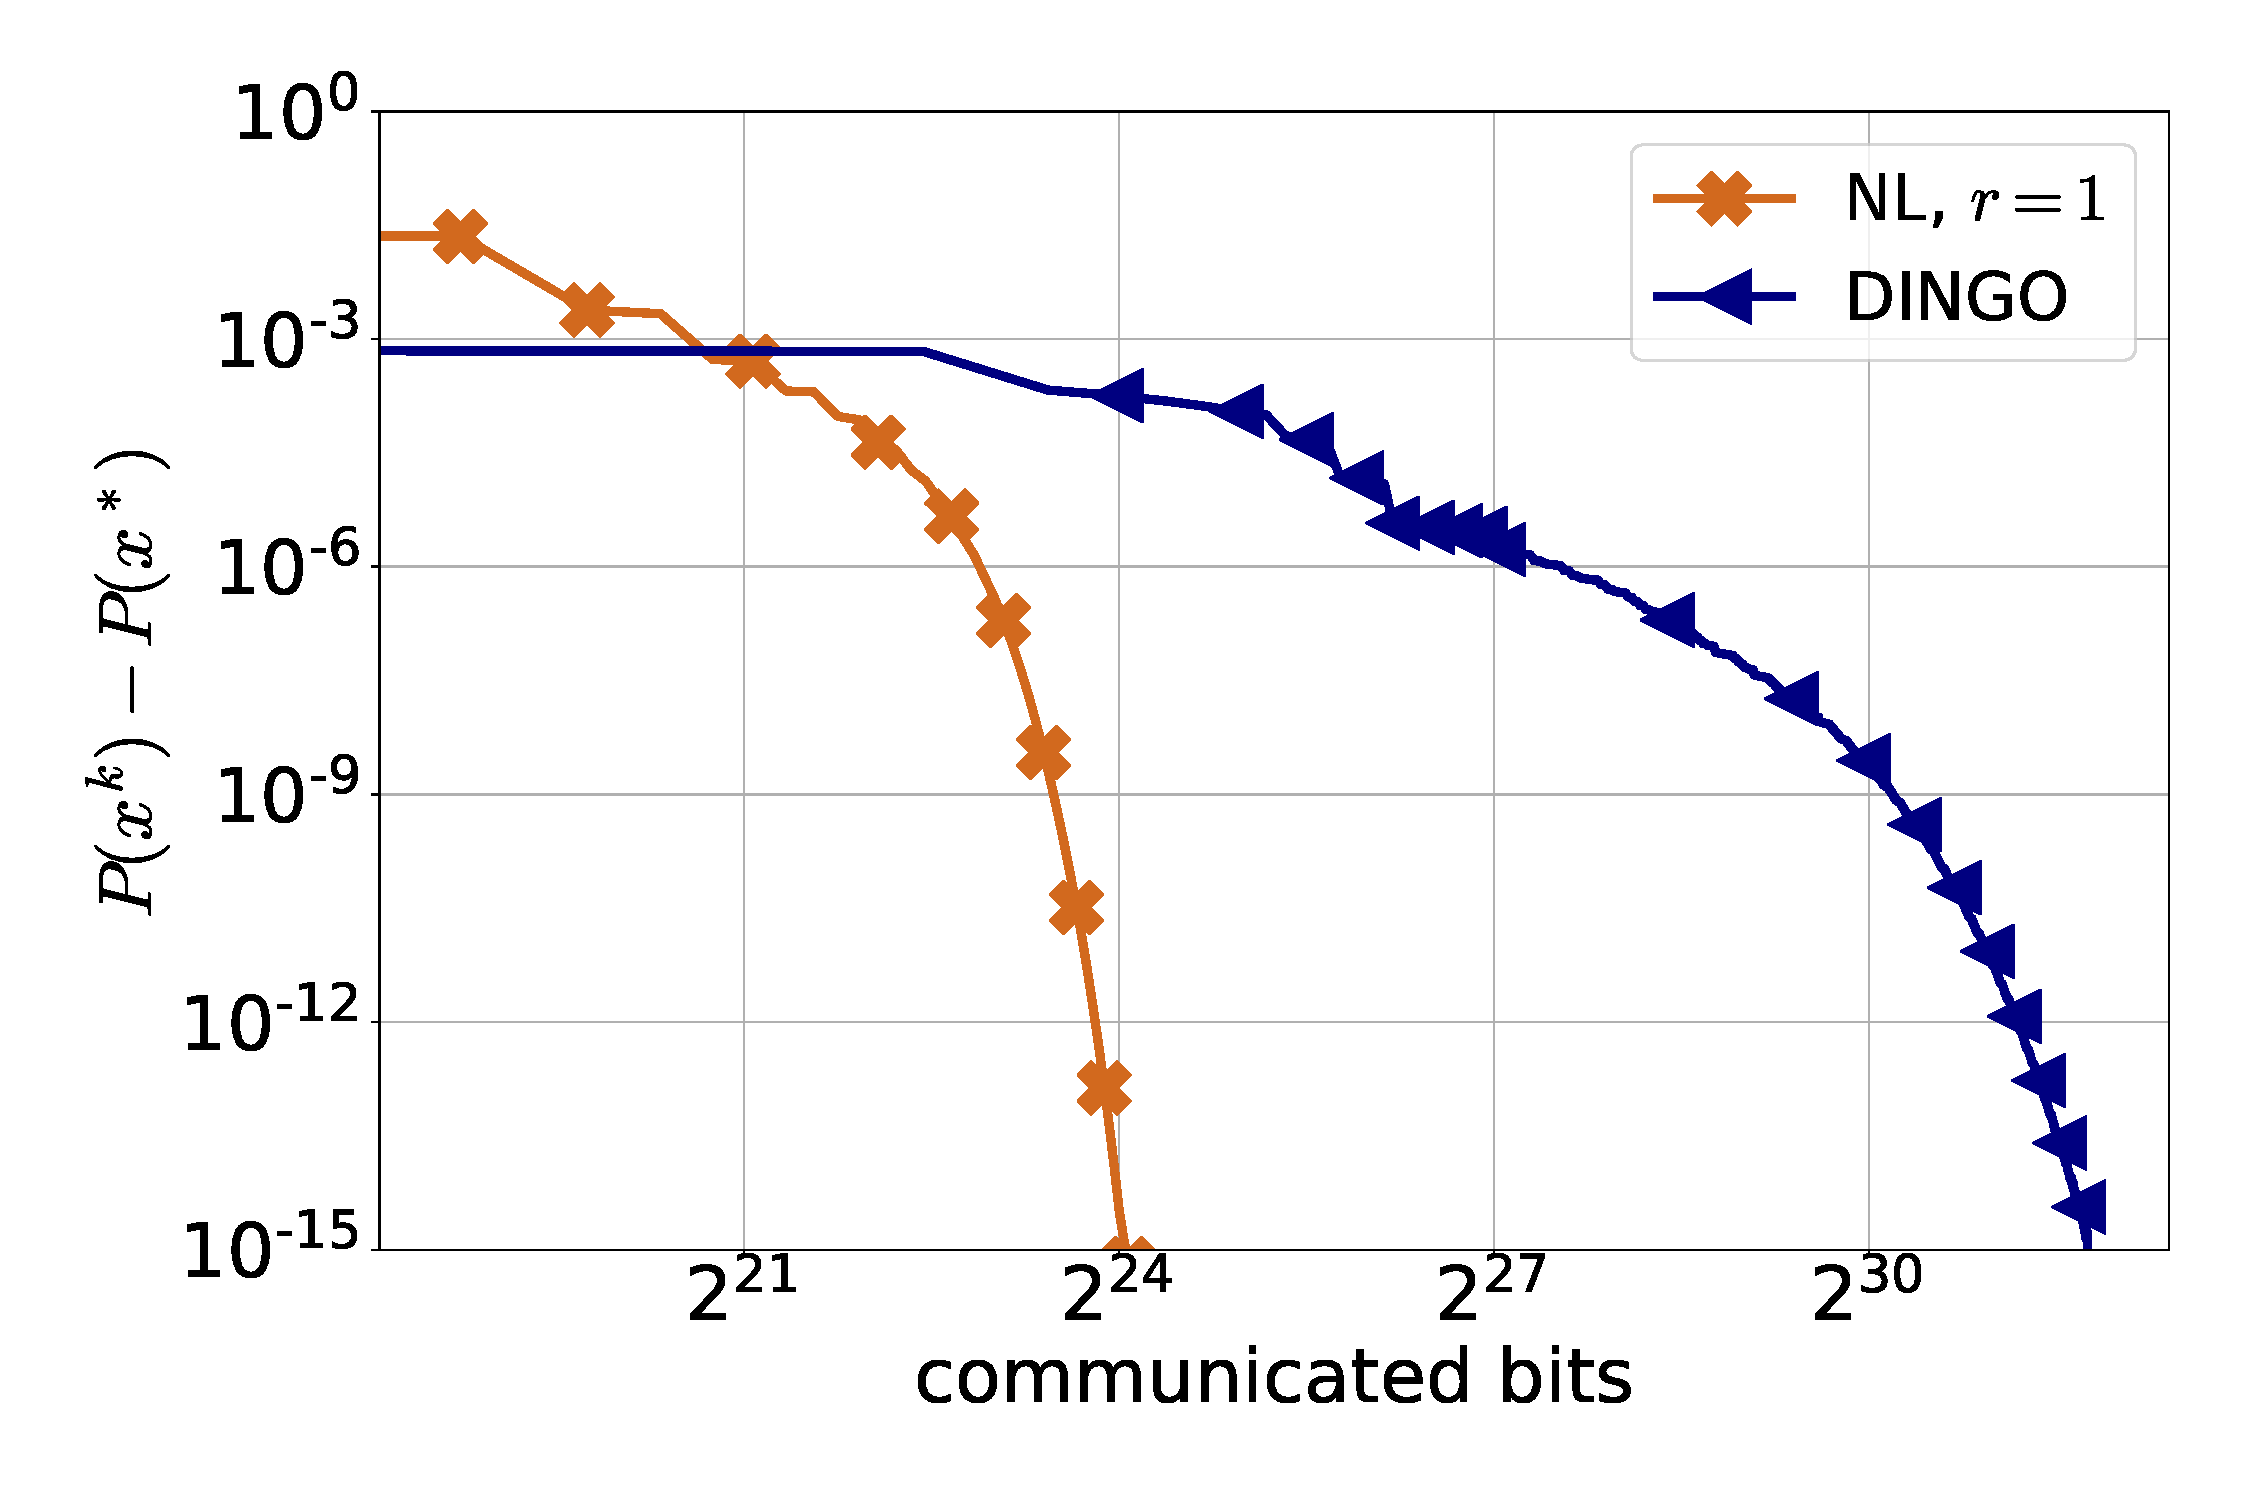
\includegraphics[width=0.3\linewidth]{phishing_nl_dingo_bits_lmb=0_00001.pdf}\\
     {\tt w8a}, $\lambda=10^{-3}$ & {\tt a9a}, $\lambda=10^{-4}$ & {\tt phishing}, $\lambda=10^{-5}$ 
\end{tabular}
    
\end{frame}

\begin{frame}{Результаты, выносимые на защиту}
\begin{itemize}
    \item Экспериментальное и теоретическое подтверждение сходимости предложенного метода;
    \item Экспериментальные данные показывают превосходство предложенного метода над существующими SOTA методами в терминах сложности коммуникаций;
    \item Придуман первый метод второго порядка в дистрибутивной оптимизации, скорость сходимости которого не зависитт от числа обусловленности функции.
\end{itemize}
    
\end{frame}





\end{document}